\documentclass[aspectratio=169]{beamer}
\usepackage[utf8]{inputenc}
\usepackage{bbding}
\usepackage[weather]{ifsym}
\usepackage{color}
\usepackage{hyperref}
\usepackage{pgfpages}
\usepackage{transparent}
\usepackage{lmodern}
\usepackage{enumitem}

\title{Transformation Workshop}

\subtitle{\fontsize{40}{40}\color{ice-blue}\SnowflakeChevron\raisebox{0.3cm}{\color{ipt-red}\selectfont~$\approx$~}\raisebox{0.2cm}{\selectfont\color{ipt-blue}\#}}


\author{Bastian Bukatz}
\institute{Innovation Process Technology}
\date{\today}


\usepackage{helvet}
\renewcommand{\familydefault}{\sfdefault}


\definecolor{ice-blue}{RGB}{162,210,223}
\definecolor{ipt-blue}{cmyk}{1,0.45,0.18,0.07}
\definecolor{ipt-red}{cmyk}{0,1,0.53,0}
\setbeamercolor{title}{fg=ipt-blue}
\setbeamercolor{frametitle}{fg=ipt-blue}
\setbeamercolor{normal text}{fg=black}
\setbeamercolor{alerted text}{fg=ipt-red}
\setbeamercolor{section in toc}{fg=ipt-blue}
\setbeamercolor{item}{fg=ipt-blue}


\usepackage{hyperref}
\hypersetup{colorlinks=true,linkcolor=ipt-blue,urlcolor=ipt-blue}

\makeatletter
\setbeamertemplate{frametitle}{
    \ifbeamercolorempty[bg]{frametitle}{}{\nointerlineskip}%
    \@tempdima=\textwidth%
    \advance\@tempdima by\beamer@leftmargin%
    \advance\@tempdima by\beamer@rightmargin%
    \hspace*{0.3cm} %%%%%%%%%%%%% For example insert shift to right
    \begin{beamercolorbox}[sep=0.3cm,wd=\the\@tempdima]{frametitle}
        \usebeamerfont{frametitle}%
        \vbox{}\vskip-1ex%
        \if@tempswa\else\csname beamer@ftecenter\endcsname\fi%
        \strut\insertframetitle\strut\par%
        {%
            \ifx\insertframesubtitle\@empty%
            \else%
            {\usebeamerfont{framesubtitle}\usebeamercolor[fg]{framesubtitle}\insertframesubtitle\strut\par}%
            \fi
        }%
        \vskip-1ex%
        \if@tempswa\else\vskip-.3cm\fi% set inside beamercolorbox... evil here...
    \end{beamercolorbox}%
}
\makeatother


\begin{document}

\usebackgroundtemplate{
\includegraphics[width=\paperwidth]{pictures/ipt_titelpage2.jpg}}
\begin{frame}
\titlepage
\end{frame}


\usebackgroundtemplate{
\includegraphics[width=\paperwidth]{pictures/ipt_standardpage.jpg}}

\begin{frame}
\frametitle{Table of Contents}
\tableofcontents
\end{frame}



\section{Ausgangslage}
\subsection{Stärken / Schwächen}
\begin{frame}
\frametitle{\subsecname\hfill\raisebox{-0.5cm}{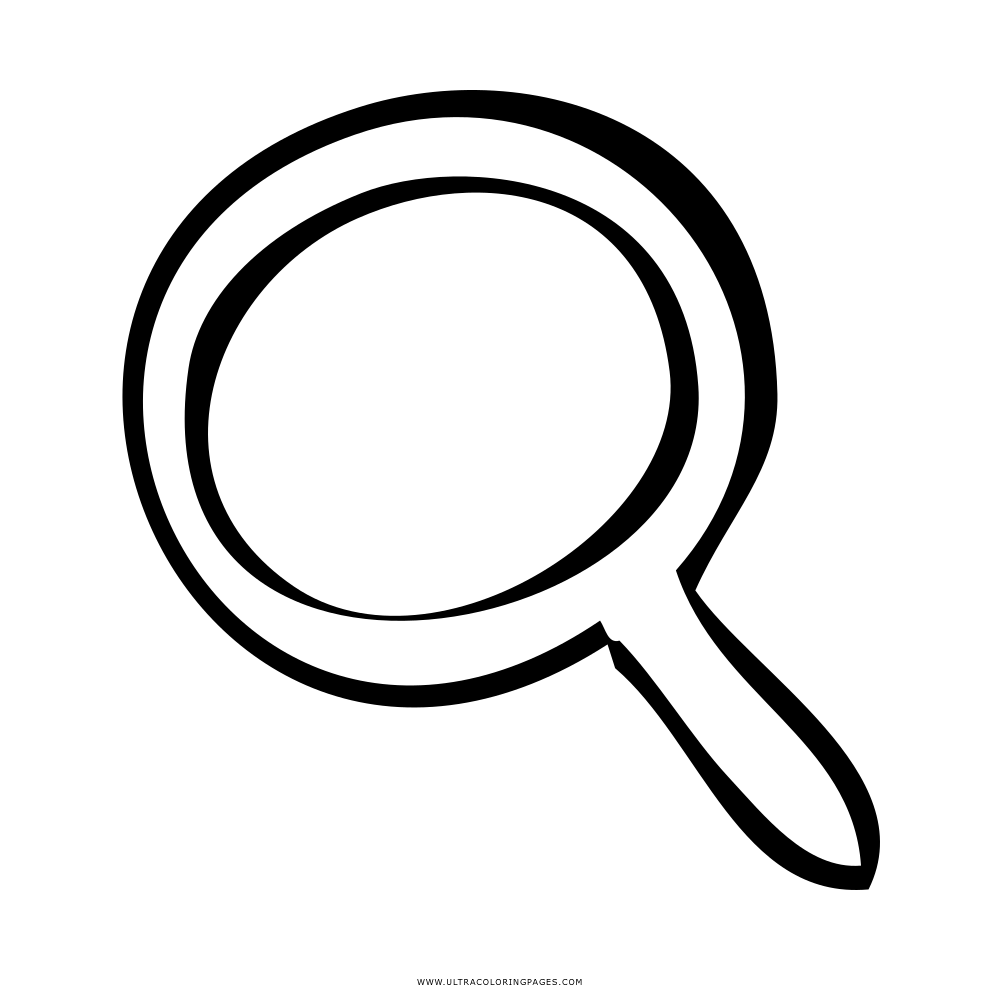
\includegraphics[height=1cm]{pictures/lupe.png}}}

\begin{itemize}[label={$\bullet$}]
\item Das IPT Change-Modell bietet einen Rahmen um Veränderungsvorhaben erfolgreich zu bewältigen
\item Das Modell basiert auf dem wissenschaftlich anerkannten "Model of Change von Kurt Lewin" sowie Elementen aus "John Kotter's 8-Step Change Model"
\item In das Modell sind die Erfahrungen unserer Consultants im erfolgreichen Begleiten von Veränderungsvorhaben eingeflossen
\end{itemize}
\end{frame}

\subsection{Need}
\begin{frame}
\frametitle{\subsecname}\framesubtitle{\secname}
\begin{itemize}
\setlength\itemsep{1em}
\item[\color{ice-blue}\SnowflakeChevron]\underline{Auftauen}\newline
Es wird eine gemeinsame Vision erarbeitet und die Organisation wird in Veränderungebereitschaft versetzt.
\item[\color{ipt-red}\selectfont$\approx$]\underline{Verändern}\newline
Es werden die richtigen Rahmenbedinungen geschaffen um die Veränderung an der Vision auszurichten.
\item[\selectfont\color{ipt-blue}\#]\underline{Stabilisieren}\newline
Nun wird dafür gesorgt, dass der noch fragile erreichte Veränderungszustand Bestand hat.
\end{itemize}
\end{frame}


\section{Pause}
\subsection{Auftauen}
\begin{frame}
\frametitle{\secname}
\centering

\includegraphics[width=0.7\textwidth]{pictures/kaffetasse.jpg}

\end{frame}

\begin{frame}
\frametitle{\subsecname}\framesubtitle{\secname}
\begin{itemize}
\setlength\itemsep{1em}
\item[\color{ice-blue}\SnowflakeChevron]\underline{Ziele}
\begin{itemize}
  \item Veränderungsbereitschaft
  \item Gemeinsame Vision
\end{itemize}
\item[\color{ice-blue}\SnowflakeChevron]\underline{Aufgaben}
\begin{itemize}
  \item Gefühl der Dringlichkeit vermitteln
  \item Führungskoalition aufbauen
  \item Ein gemeinsam anerkanntes Zielbild entwickeln
\end{itemize}
\item[\color{ice-blue}\SnowflakeChevron]\underline{Werkzeuge}
\begin{itemize}
  \item Team-Supervision
  \item Ziel-Workshop
\end{itemize}
\end{itemize}
\end{frame}


\section{Zukunft}
\subsection{Chances}
\begin{frame}
\frametitle{\subsecname}\framesubtitle{\secname}

\end{frame}

\begin{frame}
\frametitle{\subsecname}\framesubtitle{\secname}
\begin{itemize}
\setlength\itemsep{1em}
\item[\color{ipt-red}{\selectfont$\approx$}]\underline{Ziele}
\begin{itemize}
  \item Alle ziehen an einem Strang
\end{itemize}
\item[\color{ipt-red}{\selectfont$\approx$}]\underline{Aufgaben}
\begin{itemize}
\item Hindernisse aus dem Weg räumen
\item Kurzfristige Erfolge sichtbar machen
\end{itemize}
\item[\color{ipt-red}{\selectfont$\approx$}]\underline{Werkzeuge}
\begin{itemize}
  \item Teamcoaching
  \item Retrospektiven
\end{itemize}
\end{itemize}
\end{frame}

\subsection{Stabilisieren}
\begin{frame}
\frametitle{\subsecname}\framesubtitle{\secname}
Das Ziel ist erreicht und alle Teams entfalten die gewünschte Wirkung. Aber aufgepasst. Dieser neue Zustand ist noch sehr fragil. Es ist allgemein bekannt, dass Menschen in Stress-Situationen sehr schnell in alte Gewohnheiten zurückfallen. Es ist daher wichtig, den neuen Zustand zu stabilisieren indem die Teams weiter begleitet werden, bis die Veränderungen tatsächlich in der Kultur verankert sind.
\end{frame}

\begin{frame}
\frametitle{\subsecname}\framesubtitle{\secname}
\begin{itemize}
\setlength\itemsep{1em}
\item[\selectfont\textcolor{ipt-blue}{\#}]\underline{Ziele}
\begin{itemize}
  \item Der neue Zustand wir zur Normalität
\end{itemize}
\item[\selectfont\textcolor{ipt-blue}{\#}]\underline{Aufgaben}
\begin{itemize}
\item Veränderung weiter antreiben, nicht nachlassen
\item Veränderungen in der (Unternehmens-)Kultur verankern
\end{itemize}
\item[\selectfont\textcolor{ipt-blue}{\#}]\underline{Werkzeuge}
\begin{itemize}
  \item Retrospektiven
\end{itemize}
\end{itemize}
\end{frame}


\section{Wissenschaftlicher Hintergrund}
\subsection{John Kotter’s 8-Step Change Model}
\begin{frame}
\frametitle{\subsecname}\framesubtitle{\secname}
\begin{itemize}[label={$\bullet$}]
\item Gefühl der Dringlichkeit vermitteln
\item Führungskoalition aufbauen
\item Vision und Strategie entwickeln
\item Vision kommunizieren
\item Hindernisse aus dem Weg räumen
\item Kurzfristige Erfolge sichtbar machen
\item Veränderung weiter antreiben, nicht nachlassen
\item Veränderungen in der (Unternehmens-)Kultur verankern
\end{itemize}
\mbox{}
\vfill
\begin{figure}[!b]
    Kotter, J. P. (1996). \href{http://doi.org/10.1007/s13398-014-0173-7.2}{Leading Change}. Harvard Business Review, 187.
\end{figure}

\end{frame}

\subsection{Model of Change von Kurt Lewin}
\begin{frame}
\frametitle{\subsecname}\framesubtitle{\secname}
\centering
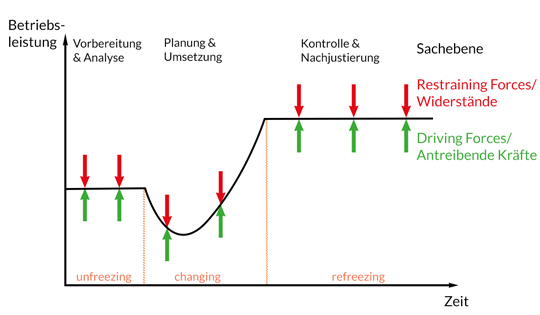
\includegraphics[width=0.7\textwidth]{pictures/3Phasen_Kurt_Lewin_web.jpg}
\vfill
\begin{figure}[!b]
  Burnes, B. (2004). \href{http://doi.org/10.1111/j.1467-6486.2004.00463.x}{Kurt Lewin and the planned approach to change: A re-appraisal}. Journal of Management Studies.
\end{figure}
\end{frame}

\end{document}
